% ============================================================
% NeurIPS 2026 Proposal — Full Revised Version
% Equivariant Temporal Sheaf Networks for Protein–Ligand
% Dissociation Kinetics
% ============================================================
\documentclass[12pt,a4paper]{article}

% --- Encoding & fonts ----------------------------------------
\usepackage[T1]{fontenc}
\usepackage[utf8]{inputenc}
\usepackage{lmodern}
\usepackage{microtype}

% --- Page geometry -------------------------------------------
\usepackage[top=2.5cm,bottom=2.5cm,left=2.5cm,right=2.5cm]{geometry}

% --- Mathematics ---------------------------------------------
\usepackage{amsmath,amssymb,amsthm}
\usepackage{bm}
\usepackage{mathtools}

% --- Tables --------------------------------------------------
\usepackage{booktabs}
\usepackage{array}
\usepackage{tabularx}

% --- Typography & lists --------------------------------------
\usepackage{enumitem}
\usepackage{xcolor}
\usepackage{mdframed}

% --- TikZ for architecture diagrams --------------------------
\usepackage{tikz}
\usetikzlibrary{arrows.meta,positioning,fit,backgrounds,shapes.geometric}

% --- Headers -------------------------------------------------
\usepackage{titlesec}
\titleformat{\section}{\large\bfseries}{\thesection}{1em}{}
\titleformat{\subsection}{\normalsize\bfseries}{\thesubsection}{1em}{}
\titleformat{\subsubsection}{\normalsize\itshape}{\thesubsubsection}{1em}{}

% --- Hyperlinks & bibliography --------------------------------
\usepackage[colorlinks=true,linkcolor=blue!70!black,
            citecolor=blue!70!black,urlcolor=blue!70!black]{hyperref}
\usepackage[round,sort&compress]{natbib}
\bibliographystyle{abbrvnat}

% --- Theorem environments ------------------------------------
\newtheorem{theorem}{Theorem}
\newtheorem{proposition}{Proposition}
\newtheorem{definition}{Definition}
\newtheorem{remark}{Remark}

% --- Shaded environments -------------------------------------
\newmdenv[backgroundcolor=blue!5,linecolor=blue!40,linewidth=1pt,
          innertopmargin=7pt,innerbottommargin=7pt,
          skipabove=8pt,skipbelow=8pt]{claimbox}

\newmdenv[backgroundcolor=orange!8,linecolor=orange!50,linewidth=1pt,
          innertopmargin=7pt,innerbottommargin=7pt,
          skipabove=8pt,skipbelow=8pt]{warnbox}

\newmdenv[backgroundcolor=green!6,linecolor=green!50!black,linewidth=1pt,
          innertopmargin=7pt,innerbottommargin=7pt,
          skipabove=8pt,skipbelow=8pt]{resultbox}

% --- Title ---------------------------------------------------
\title{%
  \textbf{Equivariant Temporal Sheaf Networks for\\
  Protein--Ligand Dissociation Kinetics}\\[6pt]
  \normalsize Benchmark $+$ Method $+$ Mechanistic Analysis
}
\author{}
\date{\today}

% =============================================================
\begin{document}
\maketitle
\tableofcontents
\clearpage

% =============================================================
\section{One-Sentence Claim and Positioning}
\label{sec:claim}
% =============================================================

\begin{claimbox}
\textbf{Central claim.}
We propose an equivariant temporal sheaf architecture that learns
geometry-aware local frame transport on molecular dynamics (MD) trajectories,
and improves protein--ligand dissociation kinetics prediction under
leakage-aware cold-start benchmarks.
\end{claimbox}

\paragraph{How to pitch this paper.}
\emph{Do not} pitch it as ``TSNN predicts residence time from short unbiased
MD.'' Pitch it as:

\begin{claimbox}
\centering
\textit{An equivariant temporal sheaf framework for learning
dissociation-relevant geometry from MD trajectories, paired with a rigorous
kinetics benchmark and mechanistic contact-level analyses.}
\end{claimbox}

Short MD is best used for pretraining and local instability forecasting;
scarce kinetics labels are reserved for fine-tuning.
That framing survives the current protein--ligand benchmarking literature,
which is now explicit about leakage, structural artefacts, and inflated
random-split performance
\citep{plinder2024,hiqbind2025,cleansplit2025,leakproofpdbbind2024}.

% =============================================================
\section{Why Now: Three Convergent Developments}
\label{sec:why}
% =============================================================

\paragraph{Large MD corpora.}
MISATO~\citep{misato2024} provides QM-refined structures with explicit-water
MD over ${\approx}20{,}000$ complexes ($>170\,\mu$s).
MDbind~\citep{mdbind2025} supplies 63{,}000 simulations with spatiotemporal
baselines (Timenucy, Videonucy) and demonstrates that full MD training reduces
bias relative to static-only learning.
MDD~\citep{mdd2024} adds 862 complexes at standardised 200\,ns.
DD-13M~\citep{dd13m2025} adds over 26{,}000 complete dissociation trajectories
for 565 complexes (${\approx}13\times10^6$ all-atom frames), making
dissociation-trajectory ML practically feasible.

\paragraph{Sheaf and topological models for biomolecules.}
Neural Sheaf Diffusion~\citep{nsd2022} introduced learnable sheaf Laplacians
for GNNs.
The 2025 physics-informed sheaf model~\citep{physicsinformedsheaf2025} links
the anisotropic sheaf Laplacian to the Hessian / normal-mode viewpoint.
Persistent sheaf Laplacians have been applied to protein
flexibility~\citep{pslflex2025} and protein--nucleic acid
flexibility~\citep{pslpna2026}.
The remaining gap---\emph{temporal sheaf transport on MD trajectories for
dissociation kinetics}---is the niche this paper targets.

\paragraph{Kinetics-focused ML.}
STELLAR-koff~\citep{stellarkoff2025} targets $k_{\text{off}}$ via multiple
ligand conformations and introduces an expanded PDBbind-$k_{\text{off}}$ set
of 1{,}197 entries.
The area is becoming competitive; novelty must come from temporal geometry
plus rigorous benchmarking.

% =============================================================
\section{The Main Trap to Avoid}
\label{sec:trap}
% =============================================================

\begin{warnbox}
\textbf{What will not work.}
A direct claim that 5--10\,ns unbiased MD alone can reliably predict
experimental residence times across broad target classes is too strong.
Treat short unbiased MD as a \emph{pretraining source} and a source of
\emph{local hazard proxies}, not as sufficient supervision for general
$k_{\text{off}}$ prediction.
\end{warnbox}

\begin{warnbox}
\textbf{Benchmarking mistake to avoid.}
PLINDER~\citep{plinder2024}, HiQBind~\citep{hiqbind2025}, and
CleanSplit~\citep{cleansplit2025} show that random-split performance can be
severely distorted by structural redundancy and train--test leakage.
Do not headline random-split results.
\end{warnbox}

% =============================================================
\section{Research Questions}
\label{sec:rq}
% =============================================================

\begin{enumerate}
  \item \textbf{Representation.}
        Does temporal sheaf transport improve dynamic protein--ligand
        representation relative to flat temporal encoders and MD-aware models
        such as Dynaformer~\citep{dynaformer2024},
        DynamicDTA~\citep{dynamicdta2025},
        DynHeter-DTA~\citep{dynheterdta2025}, and MDbind~\citep{mdbind2025}?
  \item \textbf{Prediction.}
        Can short MD prefixes predict dissociation kinetics or near-future
        local dissociation hazard?
  \item \textbf{Mechanism.}
        Do sheaf disagreement signals anticipate contact failure before
        macroscopic separation?
  \item \textbf{Generalisation.}
        Does the geometric inductive bias improve performance under cold-start
        and interaction-deleaked splits?
\end{enumerate}

% =============================================================
\section{Scientific Hypothesis}
\label{sec:hypothesis}
% =============================================================

\begin{definition}[Sheaf disagreement]
Let $\mathbf{h}_u(t)\in\mathbb{R}^d$ be the latent state of node $u$ at
time $t$, and let $\mathbf{Q}_{uv}(t)\in\mathrm{O}(d)$ be the learned
transport map from $v$ to $u$.
The \emph{sheaf disagreement} on contact $(u,v)$ at time $t$ is
\begin{equation}
  \mathcal{D}_{uv}(t)
  \;=\;
  \bigl\|\mathbf{h}_u(t)-\mathbf{Q}_{uv}(t)\,\mathbf{h}_v(t)\bigr\|^2.
  \label{eq:disagreement}
\end{equation}
\end{definition}

\begin{claimbox}
\textbf{Central hypothesis.}
Persistent growth in $\mathcal{D}_{uv}(t)$ over critical protein--ligand
contacts provides an early-warning signal for contact rupture and elevated
complex-level dissociation hazard.
\end{claimbox}

% =============================================================
\section{Concrete Architecture}
\label{sec:arch}
% =============================================================

The model has four sequential components, shown in Figure~\ref{fig:arch}.

\begin{figure}[ht]
\centering
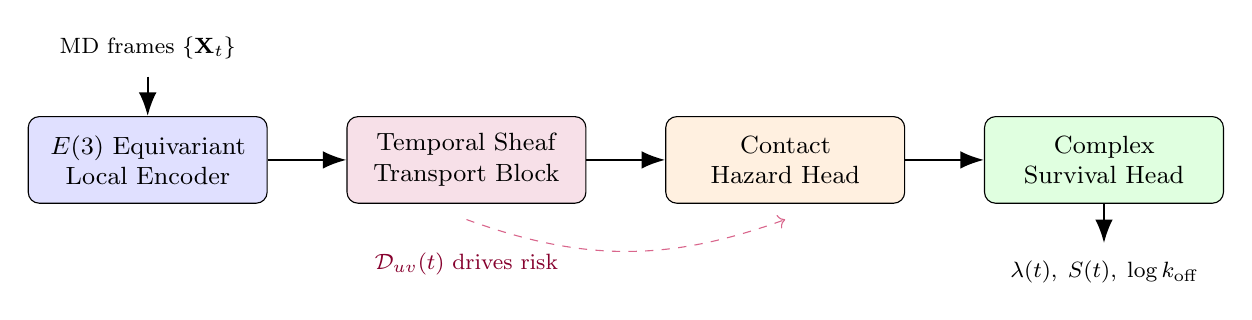
\begin{tikzpicture}[
  node distance=6mm and 10mm,
  box/.style={draw,rounded corners=4pt,fill=#1,minimum width=30mm,
              minimum height=11mm,font=\small,align=center,text width=28mm},
  arr/.style={-{Latex[length=3mm]},thick}
]
\node[box=blue!12]    (enc)   {$E(3)$ Equivariant\\Local Encoder};
\node[box=purple!12,right=of enc]  (sheaf) {Temporal Sheaf\\Transport Block};
\node[box=orange!12,right=of sheaf](chaz)  {Contact\\Hazard Head};
\node[box=green!12, right=of chaz] (surv)  {Complex\\Survival Head};

\draw[arr] (enc)   -- (sheaf);
\draw[arr] (sheaf) -- (chaz);
\draw[arr] (chaz)  -- (surv);

\node[above=6mm of enc,font=\footnotesize]{MD frames $\{\mathbf{X}_t\}$};
\draw[arr] ([yshift=5mm]enc.north) -- (enc.north);

\node[below=6mm of surv,font=\footnotesize]
     {$\lambda(t),\;S(t),\;\log k_{\text{off}}$};
\draw[arr] (surv.south) -- ([yshift=-5mm]surv.south);

\node[below=5mm of sheaf,font=\footnotesize,text=purple!70!black]
     {$\mathcal{D}_{uv}(t)$ drives risk};
\draw[->,dashed,purple!60]
     ([yshift=-2mm]sheaf.south) to[bend right=20]
     ([yshift=-2mm]chaz.south);
\end{tikzpicture}
\caption{Full model pipeline: equivariant encoding, temporal sheaf
  transport, contact hazard, and complex survival decoding.}
\label{fig:arch}
\end{figure}

\subsection{Component 1: Hybrid residue--atom graph}
\label{sec:graph}

At each frame $t$ build a local active subgraph
$G_t=(\mathcal{V},\mathcal{E}_t,\mathbf{X}_t)$ containing:
all ligand atoms; pocket residues within 8--12\,\AA\ (residue/side-chain
level, atom-level for catalytic residues); optional interfacial waters;
one support-context shell.

\paragraph{Edge types.}
Covalent and backbone; intra-pocket non-covalent (H-bond, hydrophobic,
salt bridge); protein--ligand cross-edges $\mathcal{E}^{\times}_t$;
water-mediated bridging (ablated in Section~\ref{sec:ablations}).

\paragraph{Node features.}
Coordinates $\mathbf{x}_v(t)\in\mathbb{R}^3$, atom/residue type, partial
charge, solvent exposure, side-chain torsion, and short-horizon motion
features: displacement $\Delta\mathbf{x}_v$, local RMSF, torsion change
$\Delta\phi_v$.
This mirrors the move in dynamic DTA toward explicitly dynamic features
rather than static structures alone~\citep{dynamicdta2025}.

\subsection{Component 2: $E(3)$-equivariant local encoder}
\label{sec:equivariant}

An $E(3)$-equivariant message-passing network (EGNN, SE(3)-Transformer,
or PaiNN) encodes local geometry into node states:
\begin{equation}
  \mathbf{h}_v^{(0)}(t)
  \;=\;
  \phi_{\mathrm{enc}}\!\left(
    \bigl\{
      \mathbf{x}_u(t),\,\mathbf{x}_v(t),\,d_{uv}(t),\,\mathbf{e}_{uv}(t)
    \bigr\}_{u\in\mathcal{N}(v)}
  \right).
  \label{eq:equiv}
\end{equation}
Feeding raw MD graphs directly into a sheaf layer discards 3D geometry
and places the model outside the conversation with Dynaformer
\citep{dynaformer2024} and MDbind~\citep{mdbind2025}.

\subsection{Component 3: temporal sheaf transport block}
\label{sec:sheaf}

\paragraph{Frame states and transport maps.}
For each node $v$, maintain frame matrix
$\mathbf{F}_v(t)\in\mathbb{R}^{k\times d}$ and orthogonal map
\begin{equation}
  \mathbf{U}_v(t)
  \;=\;
  \prod_{i=1}^{k} H\!\bigl(\mathbf{f}^{(i)}_v(t)\bigr),
  \qquad
  \mathbf{Q}_{uv}(t)
  \;=\;
  \mathbf{U}_v(t)^{\!\top}\mathbf{U}_u(t)
  \;\in\;\mathrm{O}(d),
  \label{eq:householder}
\end{equation}
where $H(\mathbf{f})=\mathbf{I}-2\mathbf{f}\mathbf{f}^{\top}/\|\mathbf{f}\|^2$
is a Householder reflection.

\paragraph{Key interpretation.}
$\mathbf{Q}_{uv}(t)$ aligns \emph{latent local frames}, not Euclidean
positions.
Distances, displacements, and angular geometry are provided separately
via coordinates and edge features.
This is supported by the anisotropic sheaf Laplacian interpretation
of~\citet{physicsinformedsheaf2025}.

\paragraph{Transported messages and GRU update.}
\begin{align}
  \mathbf{m}_{u\leftarrow v}(t)
  &\;=\;
  \mathrm{MLP}\!\Bigl(
    \mathbf{h}_u(t^-)\;\Vert\;
    \mathbf{Q}_{uv}(t)\,\mathbf{h}_v(t^-)\;\Vert\;
    \mathbf{e}_{uv}(t)
  \Bigr),
  \label{eq:msg}\\[4pt]
  \mathbf{h}_v(t)
  &\;=\;
  \mathrm{GRU}\!\left(
    \mathbf{h}_v(t^-),\;
    \textstyle\sum_{u\in\mathcal{N}(v)}\mathbf{m}_{v\leftarrow u}(t)
  \right).
  \label{eq:gru}
\end{align}

\subsection{Component 4: contact hazard and survival heads}
\label{sec:heads}

\paragraph{Local instability score.}
For each cross-contact $(u,v)\in\mathcal{E}^{\times}_t$:
\begin{equation}
  r_{uv}(t)
  \;=\;
  \mathrm{MLP}_{\mathrm{risk}}\!\Bigl(
    {-\mathcal{D}_{uv}(t)}\;\Vert\;
    \mathbf{e}_{uv}(t)\;\Vert\;
    \Delta\mathbf{e}_{uv}(t)
  \Bigr).
  \label{eq:risk}
\end{equation}

\paragraph{Complex-level hazard and survival.}
\begin{align}
  \lambda(t)
  &\;=\;
  \sigma\!\left(
    \mathrm{MLP}_{\mathrm{surv}}\!\!\left(
      \frac{1}{|\mathcal{E}^{\times}_t|}
      \sum_{(u,v)\in\mathcal{E}^{\times}_t} r_{uv}(t)
    \right)
  \right),
  \label{eq:hazard}\\[4pt]
  S(t)
  &\;=\;
  \prod_{\tau\le t}\bigl(1-\lambda(\tau)\bigr).
  \label{eq:survival}
\end{align}

\begin{claimbox}
\textbf{Why a survival head?}
A discrete-time survival head handles right-censored trajectories naturally
and separates the model from DynamicDTA~\citep{dynamicdta2025} and
DynHeter-DTA~\citep{dynheterdta2025}, which are affinity-oriented rather
than dissociation-oriented.
\end{claimbox}

% =============================================================
\section{Theory}
\label{sec:theory}
% =============================================================

\subsection{Stability under bounded frame drift}

\begin{theorem}[Non-expansiveness of orthogonal sheaf diffusion]
\label{thm:stability}
Let $\mathbf{Q}_{uv}(t)\in\mathrm{O}(d)$ for all $(u,v,t)$.
Then the sheaf diffusion operator $\Delta_{\mathcal{F}}(t)$ is
non-expansive:
\begin{equation}
  \bigl\|\Delta_{\mathcal{F}}(t)\,\mathbf{h}\bigr\|
  \;\le\;
  \|\mathbf{h}\|.
  \label{eq:nonexp}
\end{equation}
Moreover, if the frame drift satisfies
$\|\mathbf{U}_v(t)-\mathbf{U}_v(t')\|_F\le\varepsilon$ for all $v$,
then
\begin{equation}
  \bigl\|
    \Delta_{\mathcal{F}}(t)\,\mathbf{h}
    -\Delta_{\mathcal{F}}(t')\,\mathbf{h}'
  \bigr\|
  \;\le\;
  \|\mathbf{h}-\mathbf{h}'\|
  \;+\;
  2\varepsilon\,\|\mathbf{h}'\|.
  \label{eq:robust}
\end{equation}
\end{theorem}

\begin{remark}
Eq.~\eqref{eq:robust} guarantees that small conformational perturbations
propagate stably through the sheaf transport layer---the robustness
interpretation relevant for MD trajectories.
\end{remark}

\subsection{Sheaf disagreement as a hazard surrogate}

\begin{proposition}[Hazard upper bound via sheaf disagreement]
\label{prop:hazard}
Consider a contact process where each contact $(u,v)$ ruptures
independently at rate $\mu\,\mathcal{D}_{uv}(t)$ for constant $\mu>0$,
and where $\mathcal{D}_{uv}(t)$ is non-decreasing near rupture.
Then the aggregate dissociation hazard satisfies
\begin{equation}
  \Lambda(t)
  \;\le\;
  \mu\!\sum_{(u,v)\in\mathcal{E}^{\times}}
  \int_0^t \mathcal{D}_{uv}(\tau)\,d\tau.
  \label{eq:hazardbound}
\end{equation}
\end{proposition}

\begin{remark}
Proposition~\ref{prop:hazard} bridges $\mathcal{D}_{uv}(t)$
(Eq.~\ref{eq:disagreement}) and the survival decoder
(Eq.~\ref{eq:hazard}).
The ``simplified contact process'' assumes independent exponential
rupture rates; correlated contacts are left for future work.
\end{remark}

\subsection{Transport as local frame alignment}

Formally, the model compares neighbouring states only after alignment:
\begin{equation}
  \tilde{\mathbf{h}}_v^{(u)}(t)
  \;=\;
  \mathbf{Q}_{uv}(t)\,\mathbf{h}_v(t),
  \qquad
  \mathbf{Q}_{uv}(t)\in\mathrm{O}(d),
  \label{eq:align}
\end{equation}
which corrects systematic errors introduced by isotropic message passing
across differently oriented local frames, especially under conformational
adaptation~\citep{physicsinformedsheaf2025,hansen2019spectral}.

% =============================================================
\section{Three-Stage Training Pipeline}
\label{sec:training}
% =============================================================

\begin{figure}[ht]
\centering
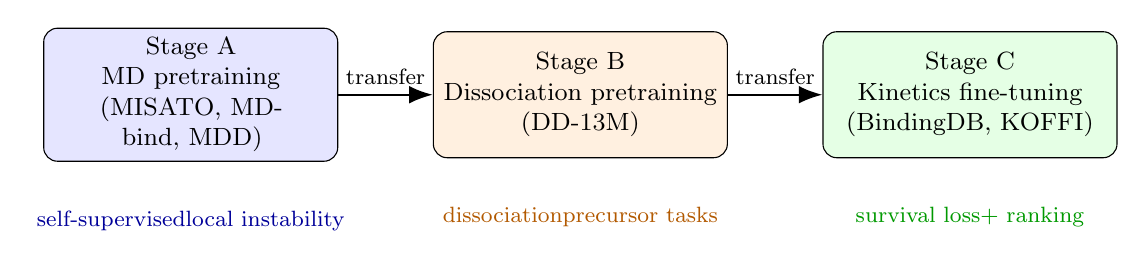
\begin{tikzpicture}[
  stage/.style={draw,rounded corners=5pt,fill=#1,minimum width=37mm,
                minimum height=16mm,font=\small,align=center,text width=35mm},
  arr/.style={-{Latex[length=3mm]},thick}
]
\node[stage=blue!10]   (a)
  {Stage A\\MD pretraining\\(MISATO, MDbind, MDD)};
\node[stage=orange!12,right=12mm of a] (b)
  {Stage B\\Dissociation pretraining\\(DD-13M)};
\node[stage=green!10, right=12mm of b] (c)
  {Stage C\\Kinetics fine-tuning\\(BindingDB, KOFFI)};

\draw[arr] (a) -- node[above,font=\footnotesize]{transfer} (b);
\draw[arr] (b) -- node[above,font=\footnotesize]{transfer} (c);

\node[below=5mm of a,font=\footnotesize,text=blue!60!black]
     {self-supervised\\local instability};
\node[below=5mm of b,font=\footnotesize,text=orange!70!black]
     {dissociation\\precursor tasks};
\node[below=5mm of c,font=\footnotesize,text=green!60!black]
     {survival loss\\$+$ ranking};
\end{tikzpicture}
\caption{Three-stage training pipeline. Each stage transfers weights
  to the next, progressively specialising from generic MD geometry
  to dissociation kinetics.}
\label{fig:training}
\end{figure}

\subsection{Stage A: self-supervised MD pretraining}

\paragraph{Data.}
MISATO~\citep{misato2024} (breadth, ML-ready loaders),
MDbind~\citep{mdbind2025} (scale, direct comparison baseline),
MDD~\citep{mdd2024} (longer runs, pipeline prototyping).

\paragraph{Objectives.}
Next-frame cross-contact prediction; contact persistence over $\Delta$
frames; local sheaf-disagreement forecasting; masked interaction-type
prediction; temporal contrastive learning across nearby windows; optional
frame-order prediction.

\subsection{Stage B: dissociation-aware pretraining}

\paragraph{Data.}
DD-13M~\citep{dd13m2025}: 26{,}612 complete dissociation trajectories,
565 complexes, ${\approx}13\times10^6$ all-atom frames.

\paragraph{Objectives.}
Contact rupture prediction; local hazard prediction
(Eq.~\ref{eq:risk}); coarse pathway classification;
time-to-escape-bin prediction; optional trajectory denoising.

\begin{claimbox}
Stage B is the strongest answer to a reviewer who says: ``your model
targets kinetics but your pretraining only uses short unbiased MD.''
\end{claimbox}

\subsection{Stage C: kinetics fine-tuning}

\paragraph{Data.}
BindingDB~\citep{bindingdb2025}, KOFFI~\citep{koffi2019}, and the
STELLAR-koff PDBbind-$k_{\text{off}}$ set~\citep{stellarkoff2025}.

\paragraph{Loss.}
\begin{equation}
  \mathcal{L}
  \;=\;
  \mathcal{L}_{\mathrm{surv}}
  \;+\;
  \alpha\,\mathcal{L}_{\mathrm{reg}}
  \;+\;
  \beta\,\mathcal{L}_{\mathrm{rank}}
  \;+\;
  \gamma\,\mathcal{L}_{\mathrm{sheaf}},
  \label{eq:loss}
\end{equation}
where $\mathcal{L}_{\mathrm{surv}}$ is the discrete-time survival NLL
(right-censoring aware), $\mathcal{L}_{\mathrm{reg}}$ is $\ell_2$
regression on $\log k_{\text{off}}$, $\mathcal{L}_{\mathrm{rank}}$ is
pairwise ranking within congeneric series, and $\mathcal{L}_{\mathrm{sheaf}}$
is a sheaf smoothness regulariser.

% =============================================================
\section{Experimental Validation Plan}
\label{sec:experiments}
% =============================================================

\subsection{Benchmark suite}

\begin{claimbox}
\textbf{Headline metric.}
Cold-protein $+$ interaction-deleaked split.
That is the setting most likely to signal seriousness to NeurIPS reviewers.
\end{claimbox}

Report all six splits:

\begin{center}
\begin{tabularx}{0.82\textwidth}{lX}
\toprule
\textbf{Split} & \textbf{Rationale} \\
\midrule
Random & Comparability with prior literature \\
Cold-protein & No close homologs in training set \\
Cold-scaffold & Scaffold-disjoint ligands \\
Pocket-cluster & Unseen binding-site families \\
Congeneric-series & Mimics medicinal chemistry SAR campaigns \\
Interaction-deleaked & PLINDER-style interaction-fingerprint threshold \\
\bottomrule
\end{tabularx}
\end{center}

PLINDER~\citep{plinder2024} provides large-scale interaction similarity
metrics; HiQBind~\citep{hiqbind2025} identifies structural artefacts;
CleanSplit~\citep{cleansplit2025} shows that removing leakage gives
more truthful generalisation estimates even when absolute numbers fall.

\subsection{Baseline families}

\paragraph{Dynamic learning baselines.}
Dynaformer~\citep{dynaformer2024}, DynamicDTA~\citep{dynamicdta2025},
DynHeter-DTA~\citep{dynheterdta2025}, MDbind Timenucy/Videonucy
\citep{mdbind2025}.
All acknowledge dynamics; none model explicit local frame transport.

\paragraph{Kinetics baselines.}
STELLAR-koff~\citep{stellarkoff2025}.
BiCoA-Net cited in prose; include in experiments if code stabilises
before submission.

\paragraph{Quality-controlled affinity baselines.}
GEMS on CleanSplit/HiQBind subsets \citep{cleansplit2025,hiqbind2025},
and a strong static equivariant scorer retrained under de-leaked splits.
Controls for the reviewer question: ``do gains come from data hygiene
rather than the sheaf model?''

\subsection{Metrics}

\begin{center}
\begin{tabularx}{0.85\textwidth}{lX}
\toprule
\textbf{Category} & \textbf{Metrics} \\
\midrule
Kinetics regression
  & RMSE, Spearman $\rho$, Pearson $r$ on $\log k_{\text{off}}$ \\
Censored prediction
  & Concordance index, integrated Brier score \\
Mechanistic early warning
  & AUROC/AUPRC for near-future contact break;
    lead time before rupture \\
Efficiency
  & Training time, inference time, memory footprint \\
\bottomrule
\end{tabularx}
\end{center}

\begin{resultbox}
\textbf{Key insight.}
A model can fail at exact $k_{\text{off}}$ prediction but still produce
a strong NeurIPS paper by succeeding at the mechanistic question:
\emph{does it identify dissociation precursors earlier than flat dynamic
baselines?}
\end{resultbox}

\subsection{What a convincing result looks like}

\begin{resultbox}
\begin{enumerate}[noitemsep,label=\arabic*.]
  \item Competitive on random split (no regression from baselines).
  \item Clearly better on cold-protein and interaction-deleaked splits.
  \item Stage B dissociation pretraining improves kinetics fine-tuning.
  \item Contact-risk head predicts rupture earlier than flat baselines.
  \item Case studies show interpretable failure modes at the binding site.
\end{enumerate}
\end{resultbox}

% =============================================================
\section{Ablations}
\label{sec:ablations}
% =============================================================

All ten ablations must appear in the main paper:

\begin{enumerate}[noitemsep]
  \item No sheaf transport: $\mathbf{Q}_{uv}(t)=\mathbf{I}$.
  \item Static frames: time-invariant $\mathbf{U}_v$.
  \item No $E(3)$ encoder (replace with RBF distance embeddings).
  \item No Stage B dissociation pretraining.
  \item No contact-level auxiliary task.
  \item No water-mediated edges.
  \item No survival head (direct $\log k_{\text{off}}$ regression only).
  \item Atom-level vs.\ hybrid residue--atom graph.
  \item Short (${\le}5$\,ns) vs.\ long (${\ge}50$\,ns) observation window.
  \item Householder depth $k\in\{1,2,4,8\}$.
\end{enumerate}

\begin{warnbox}
Running only two or three ablations will cause reviewers to call the model
under-specified.
All ten above bring the paper to a ``finished'' standard.
\end{warnbox}

% =============================================================
\section{Contribution Package}
\label{sec:contributions}
% =============================================================

\begin{claimbox}
For NeurIPS 2026 competitiveness, the paper \textbf{must} contribute all
three of:
\begin{enumerate}[noitemsep,label=\arabic*.]
  \item \textbf{Method}: equivariant temporal sheaf transport
        (Sections~\ref{sec:arch}--\ref{sec:theory}).
  \item \textbf{Benchmark protocol}: six-split de-leaked kinetics
        evaluation (Section~\ref{sec:experiments}).
  \item \textbf{Mechanistic analysis}: sheaf disagreement as a
        contact-rupture early-warning signal with binding-site
        visualisations.
\end{enumerate}
A model-only paper is high-risk.
A method $+$ benchmark $+$ interpretability paper is much more compelling.
\end{claimbox}

% =============================================================
\section{Shortest Path to a Submission-Ready Version}
\label{sec:roadmap}
% =============================================================

Priority order:
\begin{enumerate}
  \item Freeze the architecture: equivariant encoder $\to$ temporal sheaf
        core $\to$ survival head (Section~\ref{sec:arch}).
  \item Build the data pipeline on MDD first; scale to MISATO and MDbind.
  \item Add DD-13M dissociation pretraining (Stage B).
  \item Curate a high-quality kinetics fine-tuning set from
        BindingDB/KOFFI with strict de-leaking (PLINDER
        interaction-similarity threshold).
  \item Run the full six-split suite and all ten ablations.
  \item Write mechanistic case studies.
\end{enumerate}

% =============================================================
% Bibliography
% =============================================================
\clearpage
\bibliography{neurips2026_refs}

\end{document}
